%%%%%%%%%%%%%%%%%%%%%%%%%
\section{Introduction}
\label{sec:Introduction}
%%%%%%%%%%%%%%%%%%%%%%%%%

Modular self-reconfigurable robots have been proposed as one method to create general purpose robots or of arbitrary complexity in an autonomous way. These robots generally can be though of consisting of individual \textbf{modules}, which connect to other elements, either powered modules or passive structural elements, through a standardized \textbf{connector} to create a specific \textbf{configurations} in order to accomplish a designated task. The connectors themselves have several general requirements, to provide 1. some level of mechanical connection, 2. location and orientation information, 3. provide communication, or 4. provide additional connections (e.g. electrical, fluid, etc...). Many different systems have been proposed, and each system has tacked each of these connection variables in different ways, if at all. This paper focuses on the second point, looks at an overview of how location and identity information is encoded in connectors, and proposes a new method which the authors belive compares favorably with the existing state of the art.
	
The remainder of the paper is organized as follows: 
Section~\ref{sec:RelatedWork} gives an overview of related
work that pertains to modular robots, and specifically to identifying and encoding physical location information in modular connectors.
system. 
Section~\ref{sec:Hardware} presents a quick overview of the 3D Mblock modules, and then gives a detailed description of the new magnetic tag hardware and electronics.

%Next Section ~\ref{sec:Algorithims} presents the two algorithms which utilize the magnetic tags to 1. turn arbitrary configurations into %a line, and 2. form simple shapes from a line of modules.

Next, Section~\ref{sec:Experiments}
presents data characterizing the hardware and the results of
experiments with the system. 

Finally, Section~\ref{sec:Discussion}
concludes with a short discussion and ideas for future work.

\begin{figure}[htb]  

  \centering
  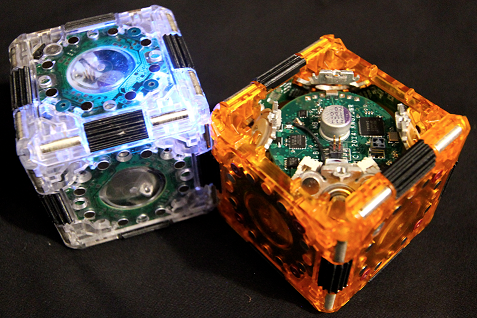
\includegraphics[width=3.4in]{Figures/cover.png}

  \caption{M-Bocks modular robots with connections illuminated with onboard LEDs}
    
  \label{fig:cover}    
\end{figure}